\section{Porovnání metod pájení přetavením z pohledu přestupu tepla}
-výhody a nevýhody jednotlivých metod se zaměřením na výrobu a opravu elektronických sestav

\textbf{Pájení přetavením} spočívá v nanesení pájecí pasty na pájecí plošky desky plošného
spoje, na kterých mají být vytvořeny pájené spoje, pak osazení součástek na desku tak,
aby jejich vývody, které mají být připájeny byly osazeny na připojovací plošky s
nanesenou pájecí pastou a následné přetavení pasty průchodem desky píckou s
vhodným teplotním profilem.

Podle způsobu ohřevu se rozlišují následující metody pájení přetavením:
\begin{itemize}
\item pájení infračerveným zářením (krátce nazývané pájení infraohřevem),
\item pájení horkým vzduchem nebo plynem (konvekční ohřev),
\item pájení v kondenzovaných parách (krátce nazývané pájení kondenzační),
\item pájení laserem,
\item pájení vyhřívaným nástrojem (někdy nazývané pájení impulsní),
\item pájení na horké desce nebo pásu
\end{itemize}

\begin{figure}[h]
   \begin{center}
     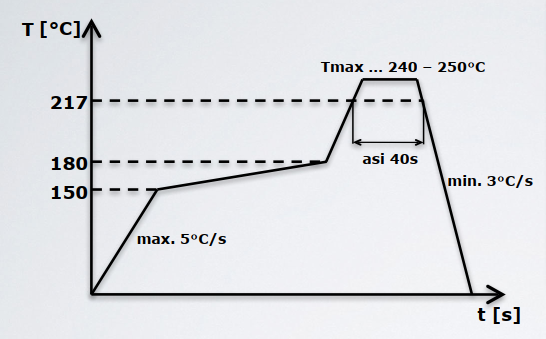
\includegraphics[scale=0.6]{images/Profil.png}
   \end{center}
   \caption{Pájení přetavením, horkým vzduchem-profil}
\end{figure}
